\documentclass{article}
\usepackage{fontspec}
\usepackage{xeCJK}
\usepackage{graphicx}
\graphicspath{ {../} }
\usepackage[margin=1in]{geometry}
\usepackage[default]{sourcesanspro}
%apparently can only use this CJK font?
\setCJKmainfont{Noto Serif CJK TC}

%info
\title{Introduction To Artificial Intelligence: Homework 1 Report}
\author{Andres Ponce(彭思安)\\
0616110}
%%%

\begin{document}
\maketitle
\section{Introduction}
	The first assignment for the course involved a chess board, and placing a knight 
	on that board. Given a starting and ending position, how do we move the knight
	along the ``best" path from the start to the finish? Using several of the methods
	described in the textbook, the task focused on comparing the performance of each one.
	Some criteria may include: completeness, time and space complexity, among other general
	observations.
\subsection{Breadth-First-Search}
	The first algorithm to be implemented was the classic Breadth-First-Search. In general,
	this algorithm keeps a ``frontier" data structure where to-be-expanded nodes are stored.
	Every iteration, we pop a node from this set and examine its children. Since we can move 
	by either $(\pm1 , \pm2)$ or $(\pm2, \pm1)$, every node has a possible 8 children.

	In this implementation, we first check the validity of the specific child node(i.e. if it 
	has already been explored), and if we have not encountered it and is withing the board bounds, 
	we add it to the frontier list, implemented here by \texttt{std::list<Node*>}. If we already explored
	a node,then we already know it does not contain a shortest path, otherwise the algorithm would have
	halted already. 

	To store the individual nodes information, we use a special \texttt{struct Node}, 
	which essentially just stores the node's correspondent x and y values in the board. Then, a quick 
	hash function can turn the x and y values into the index in the node array.

	Breadth-First Search appears to not be the most efficient algorithm to use as is, unless we add
	some form of heuristic when we choose which nodes to explore. Our algorithm will eventually reach 
	the target node, however given a large enough board the time would likely be prohibitive. Since the
	branching factor is 8, since we can make 8 possible moves at every node, the worst-case time complexity
	is $O(d^{8})$, where $d$ is the depth of the solution path.
\subsection{Depth-First-Search}
	For depth-first-search(DFS), we first carry out a thread to the end, and as we are left without valid 
	states to move on to that we start backtracking up the chain. On average, it tends to be slower than
	BFS, since we can explore a large amount of nodes before getting to the target if the target is near
	the starting point. However, the \textit{memory} requirements are quite lower. This is because at any 
	point, only the nodes on the current search path are kept in memory -- the ones we have to search --
	rather than all the nodes at a given level such as BFS. 

	
	From some of the sample tests, DFS resulted in sometimes significantly longer search paths,
	since it would search for paths that lead to dead ends.

	Depending on the problem, DFS would probably not be the most ideal search algorithm. These two first
	algorithms usually have no heuristic to select nodes, so considerable time may be spent on nodes
	that ultimately have no bearing on the final result. Thus, uninformed algorithms in general might
	not be the wisest move. 
	
	An interesting experiment or topic for further discussion given enough time might be 
	to check the actual average difference between random points on the board. 
\subsection{Iterative Deepening Search}
	Iterative Deepening Search, sometimes referred to as \textit{Iterative Deepening Depth-First Search},
	attempts to combine the useful properties of BFS and DFS in one single algorithm. First, we set a limit
	on the depth of the solution, and call a depth-first search on the starting node. Thus, whenever we find
	the solution node, it should be done using the least amount of ndoes possible.

	Every time we don't find the solution node, we increase the limit and try again. This might result
	in the top nodes of the search tree being generated often, however the difference still turns out not
	to be too great, since most nodes reside in the lower levels of the search tree(assuming constant 
	branching factor). Even though the 
	asymptotic running time remains $O(b^{d})$ (same as BFS), the memory complexity is that of DFS $O(bd)$.
	For uninformed strategies with an unknown solution depth, IDS might be the best choice since like DFS
	for a finite space, it is guaranteed to find the solution becuase of the optimality property.

	For our implementation, we use a helper function, since we recursively call the helper function. When first
	entering the helper function, besides from just checking whehter we are at the target, we also have to check
	whether the limit has been reached. Other than that, we proceed in a very similar manner to DFS.

\subsection{A* Search}
	The a* algorithm usually turns out to be one of the most effective search algorithms, since we 
	use a heuristic to make a decision on which nodes to expand. The algorithm itself is relatively 
	straightforward: for every node, we keep track of three variables $f, g,$ and $h$.  $g$ is the 
	cost of getting to node $n$, while $h$ is the (estimated) cost of arriving at the solution node. 
	Then, for each node $f = g + h$. From the child nodes, we choose one that has a lower $f$ cost than
	its parent. 

	This is where the problems begin. Due to the unconventional movement of the knight in chess, 
	the program does not find the correct answer (and sometimes no answer at all) when we have to make
	a move away from the target, to a node that is actually \textit{farther away} from the target node
	than the one we are currently in right now. For example, the sample problem involves going from 
	$(0, 0)$ to $(2, 2)$. In this case, the program would move to $(2, 1)$ and then get stuck because
	the best move is actually one that is farther away from $(2, 2)$, i.e. a node with a higher $f$ value.

	Adapting this algorithm this situation would most definitely be an interesting research question. 
	A* remains widely used in many industries, from computer vision to video games, due to its efficiency
	and correctness. Since we only expand nodes that grant a better chance of arriving at a target, then
	we can overall expand fewer nodes.

	In this implemenation, if the target node can be reached directly without going to a further point, 
	then the algorithm will reach the target node with fewer expanded nodes than with an uninformed 
	search. 
\subsection{Iterative Deepening A* Algorithm}
	This algorithm attempts to mix the Iterative Deepening algorithm while using a heuristic similar
	to the A* algorithm. We keep incrementing the bound on the node that we call the main search
	function on. However, instead of this bound coming from the depth of the search process, we
	use the nodes $f$ value. The main algorithm, \texttt{IDA\_STAR\_search} function, returns either
	if the node is found or if there is no possible path. 

	Similar to regular A*, if the heuristic we use is admissible, meaning it never underestimates
	the distance to the target node (which the sample heuristic in \texttt{Prog1.pdf} does not). 
	Thus, at every iteration the $f$ values of the nodes will not exceed the previous node's 
	$f$ value. Therefore, every node we select will have value at most the parent's $f$ value. 
	This guarantees that the optimal node will actually not be overlooked due to the estimation
	using the heursitic function. 

	However, the potential benefit of IDA* comes in memory utilization, since there is no need
	to keep a list of the nodes that we will explore as is the case in A*. In A*, the nodes were 
	checked against the Open set to see if we were duplicating nodes. This ensured that nodes were
	only expanded once. IDA* does not utilize this approach, so some nodes might be expanded 
	multiple times during the recursion process.


\section{Results}
	Below are some of the results obtained from the testing on the board. Using a standard board 
	of 8 rows  and columns, we tested the amount of expanded nodes going from $(0, 0)$ to $(2, 2)$
	as in the example, and then proceeded to test on a $16x16$ board going from $(0, 0)$ to $(7, 7)$
	and $(0, 0)$ to $(15, 15)$.

	\begin{center}
		\begin{tabular}[c]{|l | l | l | l | l | l |}
				\hline
				Route & BFS & DFS & IDS & A* & IDA* \\ \hline
				(8x8)(0, 0)->(2,2) & 83 & 25 & 55 & 6 & 2\\ \hline
				(8x8)(0,0)->(7,7) & 583 & 68 & 10 & 24 & 10\\ \hline
				(16x16)(0,0)->(7,7) & 925 & 101 & 136 & 42 & 111\\ \hline
				(16x16)(0,0)->(15, 15) & 65809 & 259 & 18 & 634 & 18\\ 
				
				\hline
		\end{tabular}
	\end{center}

	As shown, some of the results are surprising. While some may be attributable to poor implementation,
	however, with the amount of nodes that some visit, even if momentarily, can be quite large. For the BFS,
	we check all the descendants without any sort of heuristic, so larger numbers are not 
	too unexpected. 

	The ease of getting to some of the testing nodes might also play a part in the pathfinding. 
	For example, sometimes we need to ``snake" around the board until we reach the target node, even if 
	the algorithm is still relatively close to the target node. For the informed algorithms, there are
	usually less nodes required to arrive at the destination. As mentioned, for the informed search 
	algorithms there might be some problems if we have to search a node that is farther from the target
	node because the heuristic might cause that node to be overlooked. However, when we do get a 
	solution, it usually requires considerably less nodes than an algorithm such as BFS.

\section{Lessons}
	The biggest personal takeaway from this assignment was the sheer difference between informed and 
	uninformed searches. Spending valuable time expanding nodes that do not influence the final 
	result made the optimal path take considerably longer to compute. However, the problem was 
	solvable even with a relatively straightforward approach such as BFS and DFS. A* would take 
	considerably fewer nodes, usually less than 10 expansions. The total $f$ values would quickly 
	get very small,which means that the algorithm was moving in a targetetd manner towards the
	target node.

	The actual implementation of the algorithms also proved useful. Although I had already 
	implemented most of them in previous courses, this time finding a better approach to writing the
	code took more priority. Also, even though the small changes from algorithm to algorithm, or the
	way some of the algorithms tested utilize ideas from the other algorithms showed how even small 
	tweaks might influence the algorithms. Then, combining ideas from the two algorithms can sometimes
	also be applied to situations with different constraints. For example, IDS and IDA* combine 
	and build upon DFS and A*, respectively.

	The ideas behind graph search are applicable in an incredible wide range of areas, such as 
	GPS services video games, and making game-playing adversaries, to name a few examples. One 
	possible area of future research might include making an agent that can intelligently play 
	some sort of game, now knowing how some of the major algorithms compare to each other. 
\section{Code Images}

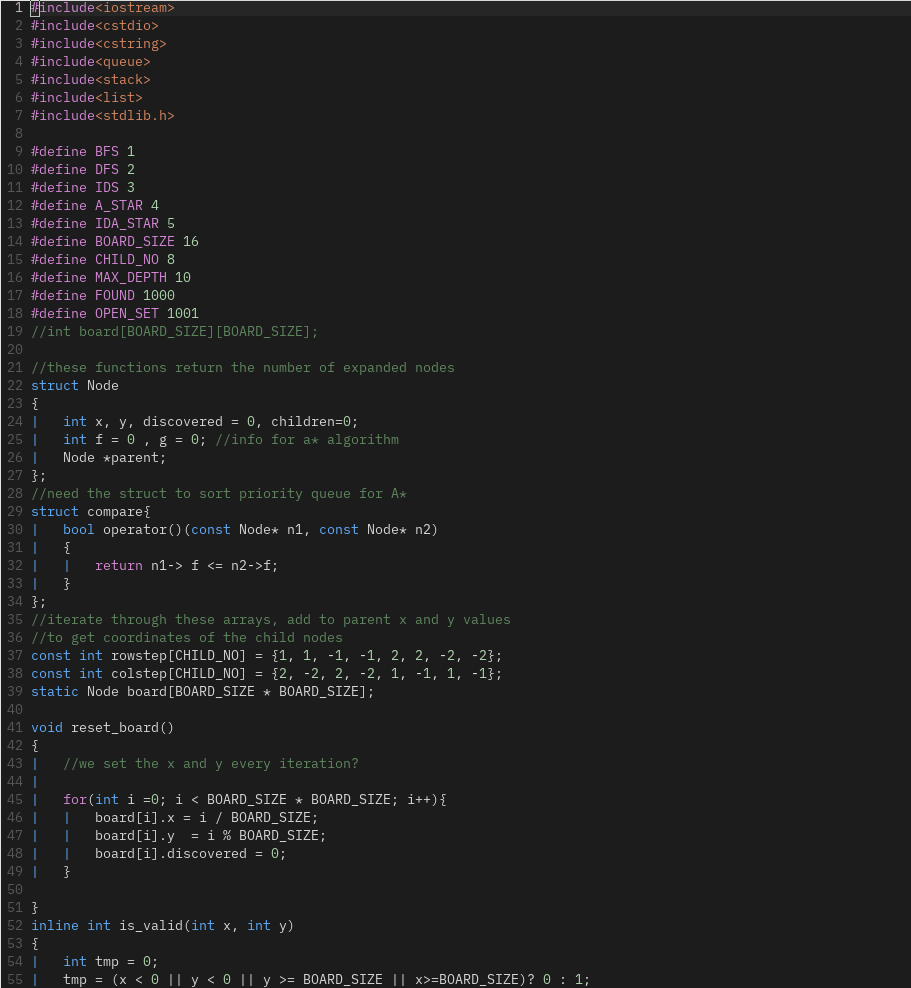
\includegraphics[scale=0.5]{sc1.png}

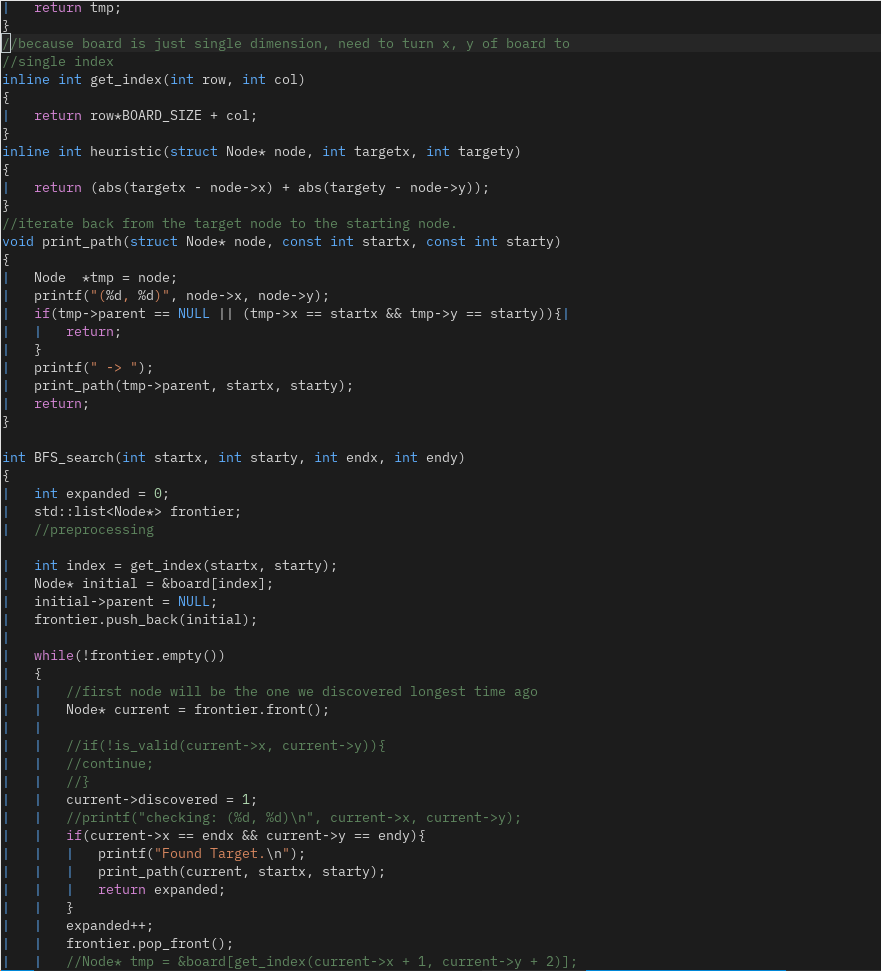
\includegraphics[scale=0.5]{sc2.png}

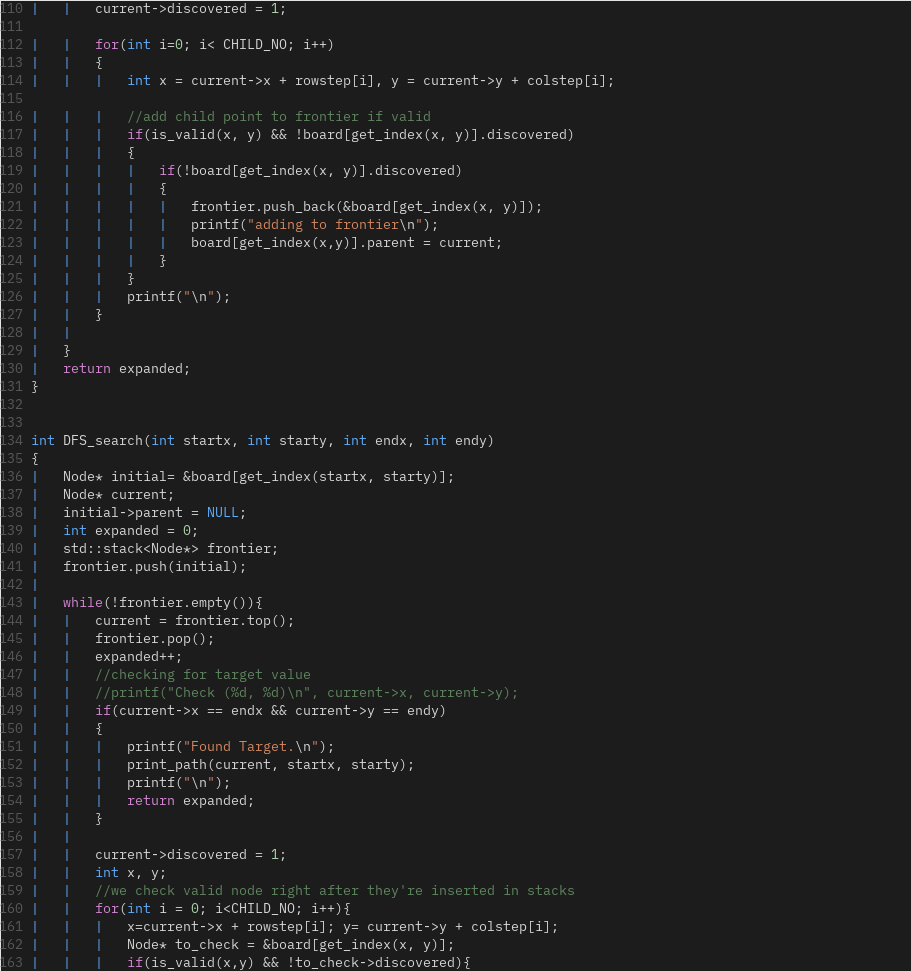
\includegraphics[scale=0.5]{sc3.png}

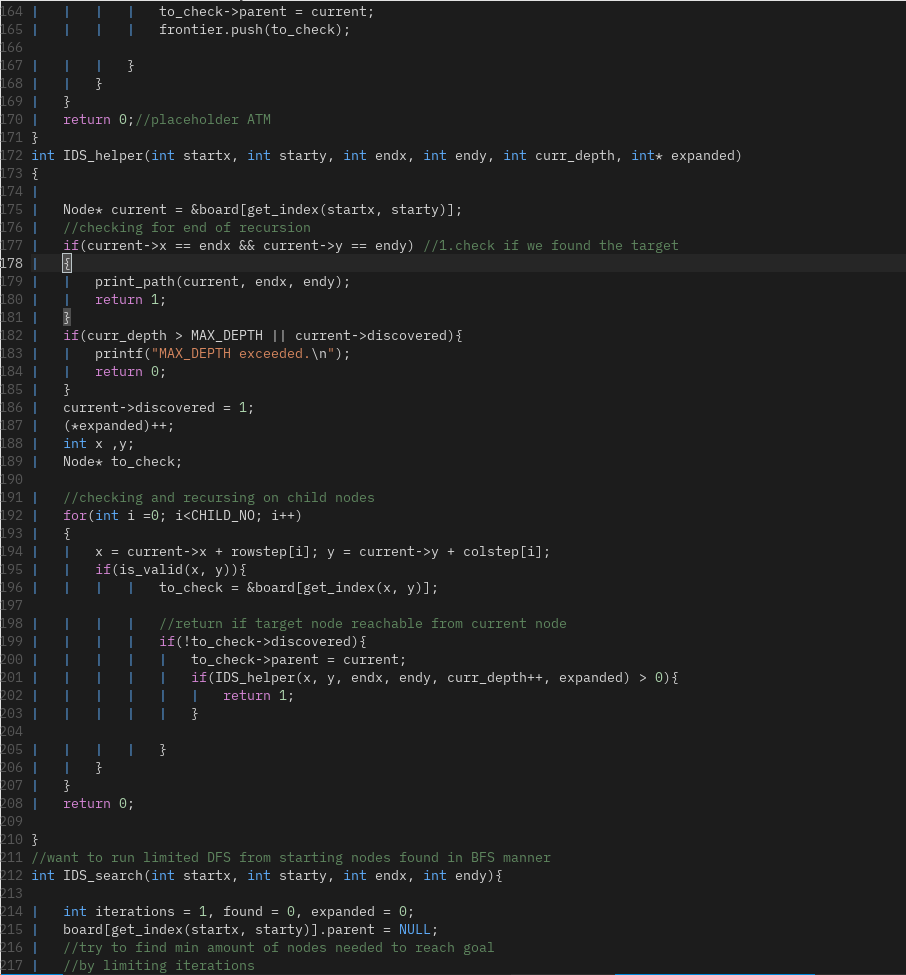
\includegraphics[scale=0.5]{sc4.png}

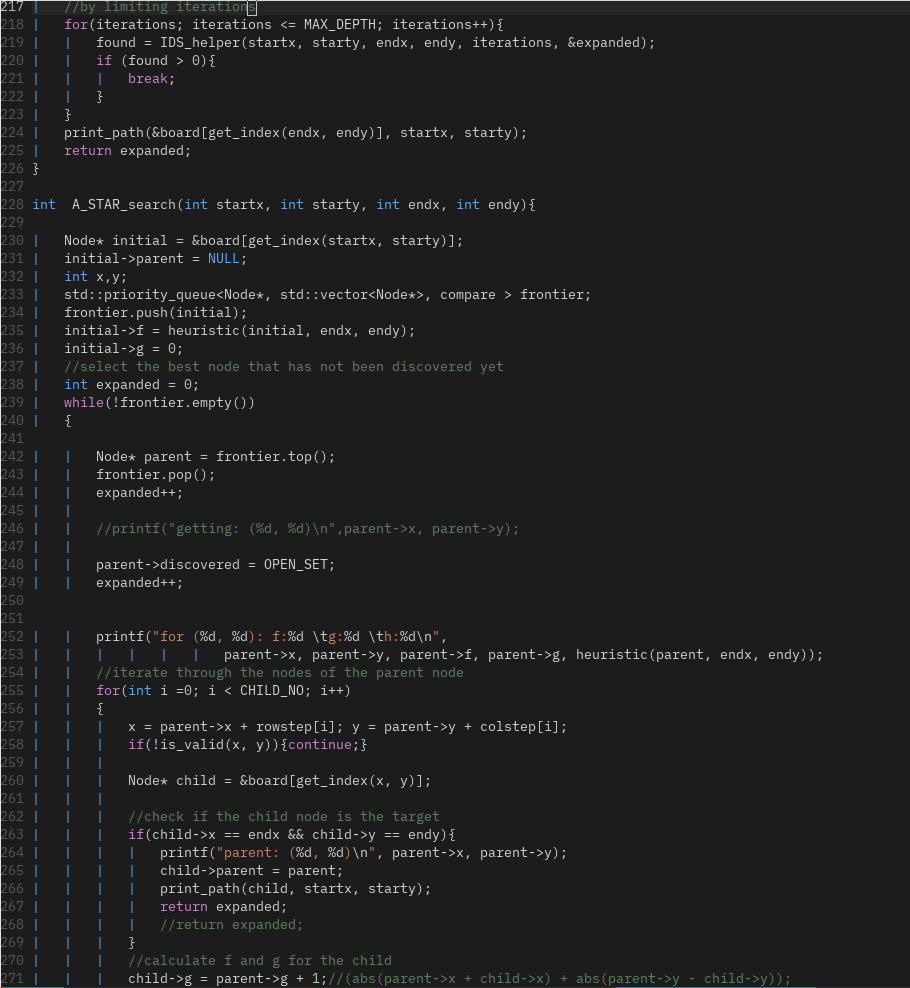
\includegraphics[scale=0.5]{sc5.png}

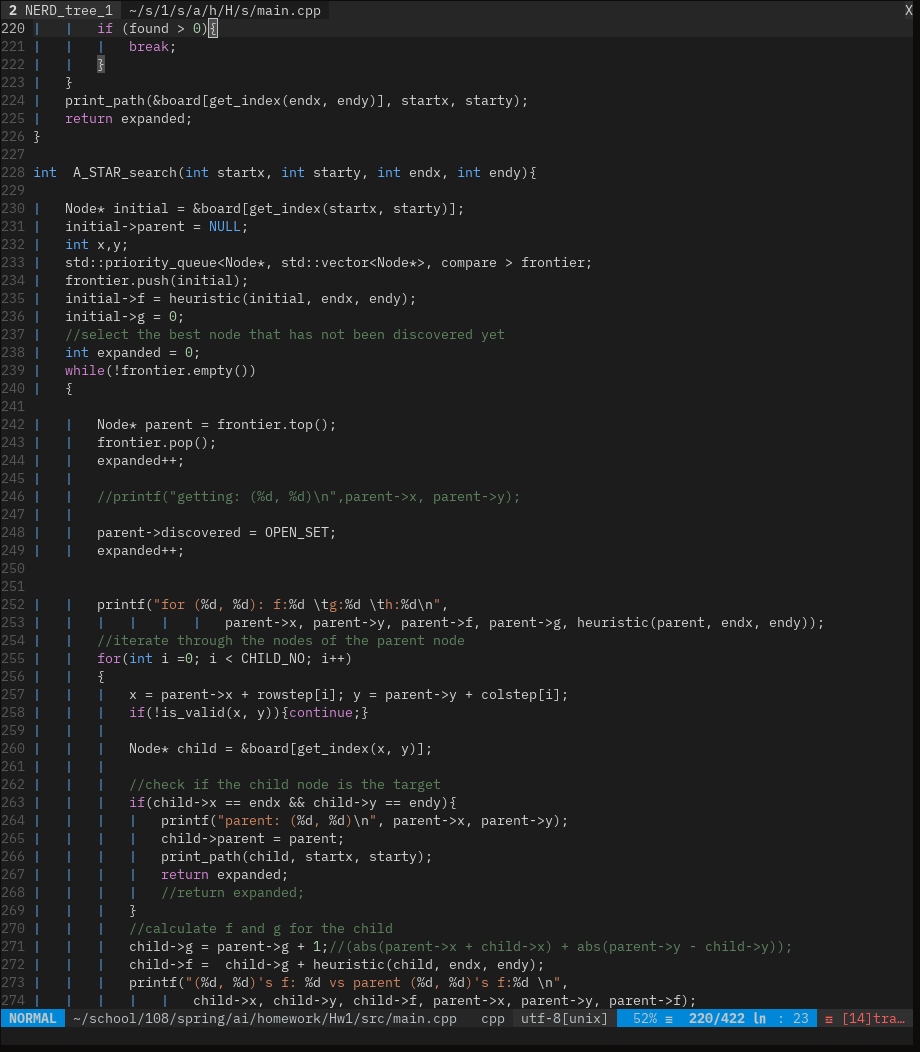
\includegraphics[scale=0.5]{sc6.png}

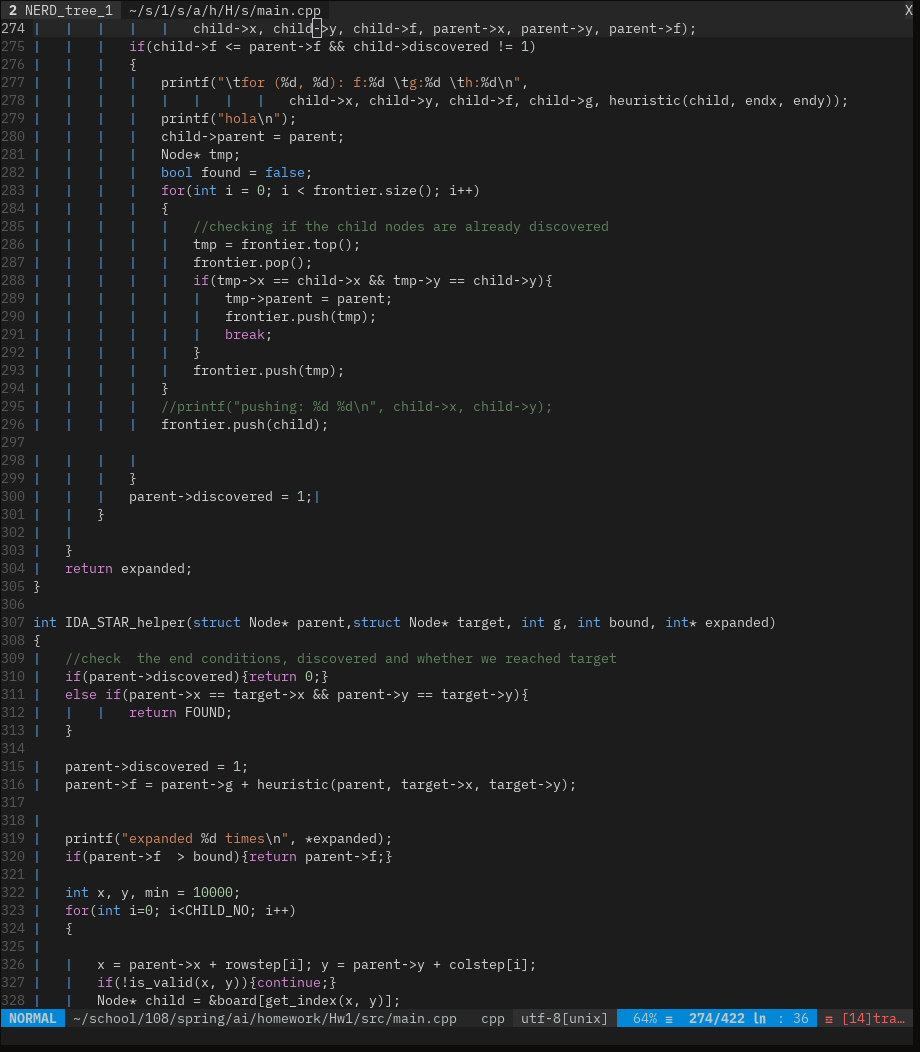
\includegraphics[scale=0.5]{sc7.png}

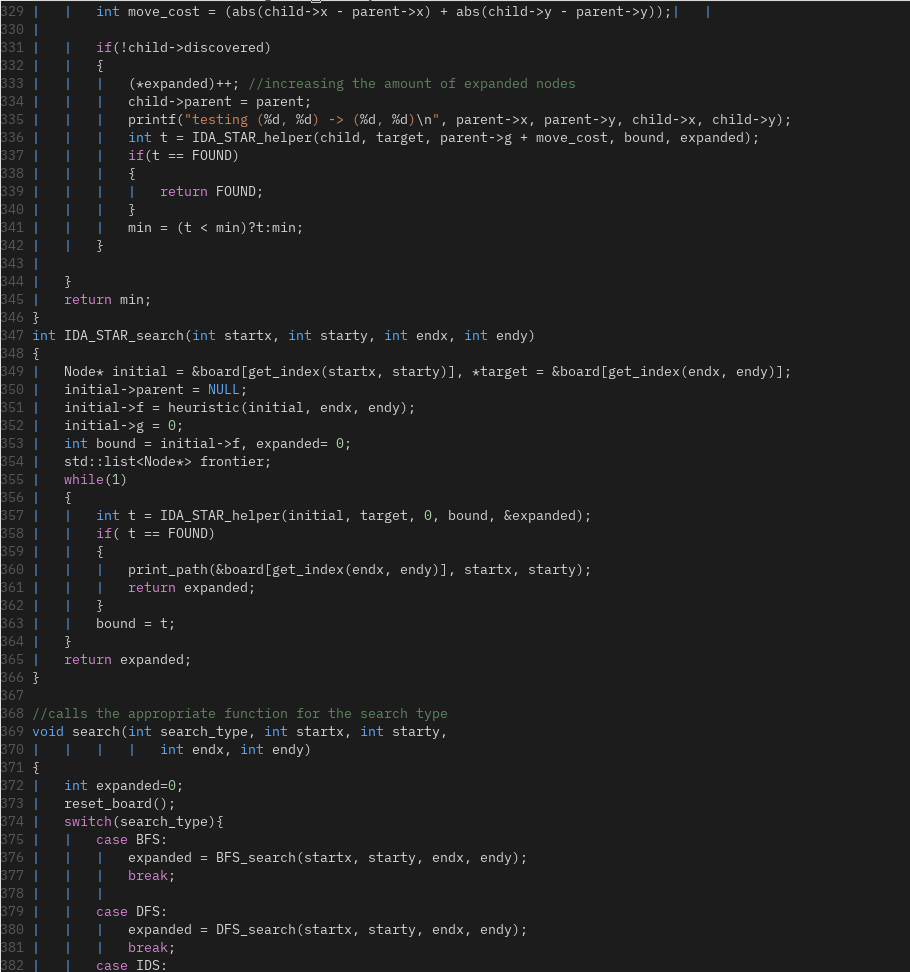
\includegraphics[scale=0.5]{sc8.png}

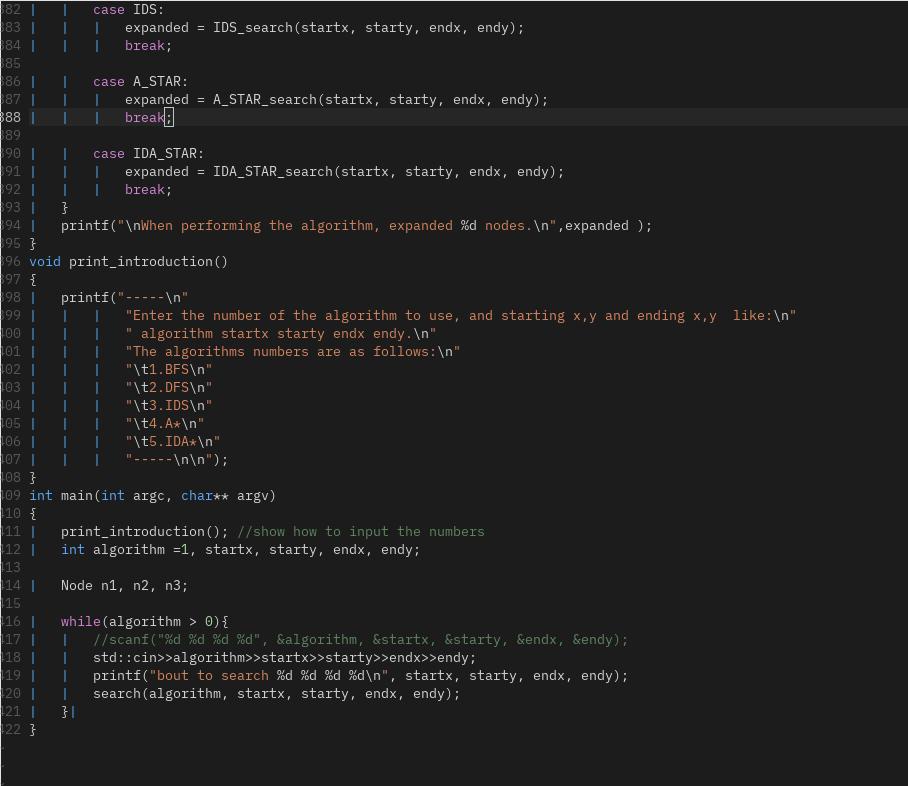
\includegraphics[scale=0.5]{sc9.png}

\end{document}
